\chapter{Implémentation}
Durant la réalisation de ce projet, nous avons essayé d’utiliser différents
outils de développement, d’une part afin de rendre la tâche de la
réalisation plus facile, d’autre part pour que notre système soit robuste et
répond parfaitement a nos besoins , et que nos interfaces soient claires et
faciles à utiliser.
\section{Architecture de l'application}
Cadorim est une application embarquée qui se connect à un serveur de base de données distant, via Internet, afin de récupérer les données, Ce qui necessite aussi l'intégration d'un serveur web entre l'application client et le serveur de bases de données.
D'où larchitecture de notre application est à 3 niveaux, elle est partagée entre;
\begin{enumerate}
	\item \textbf {L'application mobile (IOS ou Android) : }  Ce le client qui demande les ressources.
	\item \textbf{Le Serveur Web :} Vue que les données serons communiquées entre deux environnements hétérogènes, le rôle principale du serveur web est de gérer la communication entre le client (Android ou IOS) et le serveur de données.
	\item \textbf{Le serveur de base de données:} fournis les données au serveur web.
\end{enumerate}

\begin{figure}[h!]
	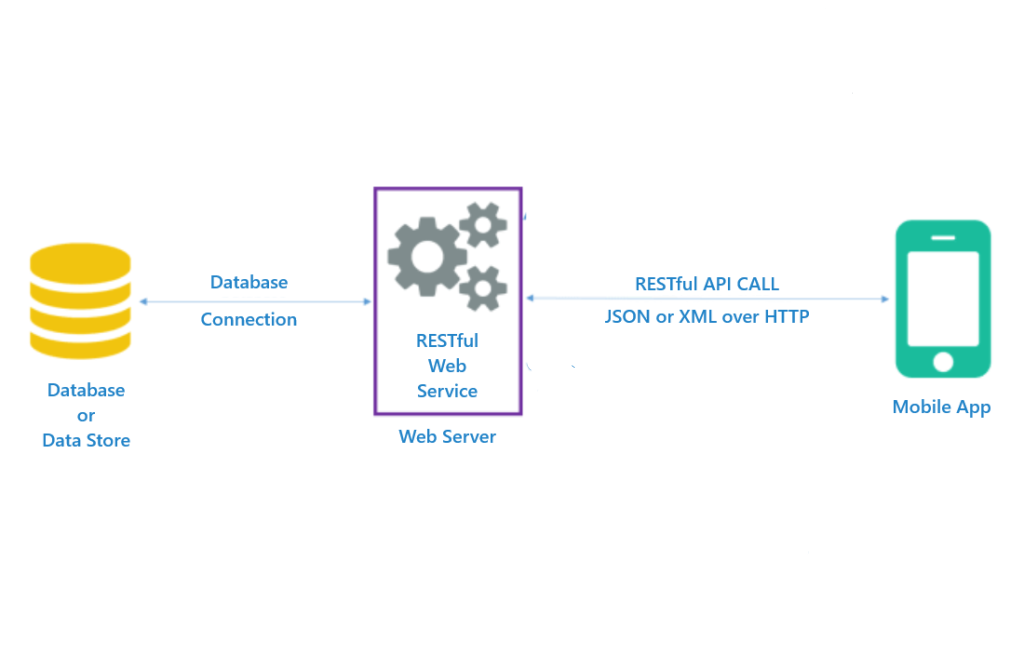
\includegraphics[width=17cm, height=10cm]{./Template LaTeX/Images/architect_after_edit.png}
	\caption{Architecture logicielle de l’application.}
	\label{fig:birds}
	
	
\end{figure}
\newpage
\section{Interfaces graphiques}
Les interfaces utilisateur doivent respecter les heuristiques d'utilité pour permettre à l'utilisateur un accès facile à ces interfaces afin de garantir une bonne compréhension des fonctionnalités de l'application. Nous présentons ici les interfaces les plus significatives de l'application.
\subsection{Interfaces d'acceil}

L'utilisateur du Cadorim avant d'être invite à consulter les services de l'application, doit 
choisies leur lange avant qu'il pass a l'interface suivante.

\begin{figure}[!ht]
	\centering
	\begin{subfigure}{0.3\textwidth}
		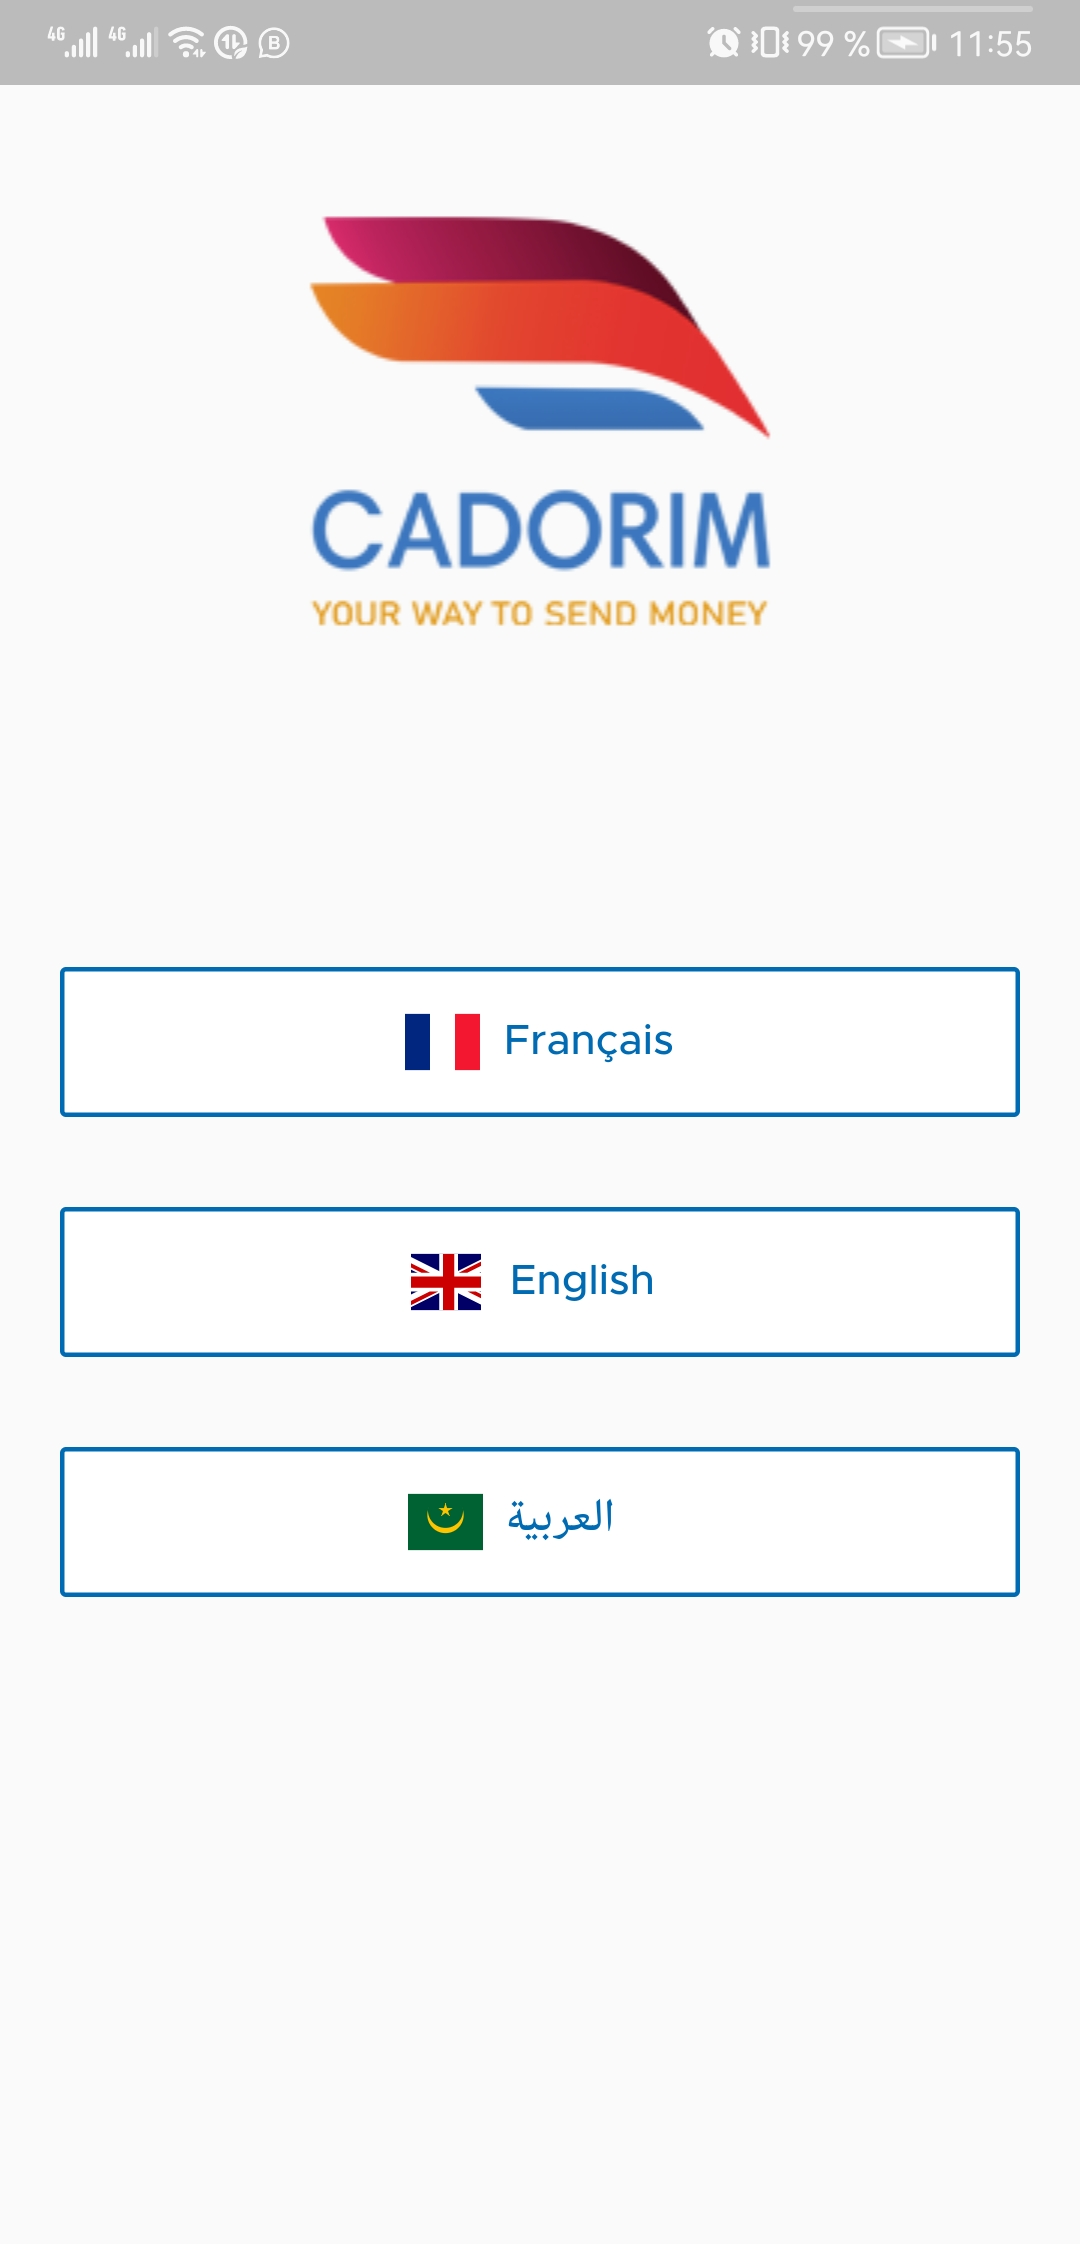
\includegraphics[width=\hsize, valign=m]{./Template LaTeX/Images/1.jpg}
		\caption{Choix de lange}
		\label{fig.SICAPI}
	\end{subfigure}
	\qquad\tikz[baseline=-\baselineskip]\draw[ultra thick,->] (0,0) -- ++ (1,0);\qquad
	\begin{subfigure}{0.3\textwidth}
		
\includegraphics[width=\hsize, valign=m]{./Template LaTeX/Images/2.jpg}
		\caption{Interfaces Accueil}
		\label{fig.painel_sicapi}
	\end{subfigure}
	\caption{Interfaces d'acceil}
	\label{fig.sicapi}
\end{figure}
\begin{comment}
	
\begin{figure}%
	\centering
	\subfloat[\centering choix de lange ]{{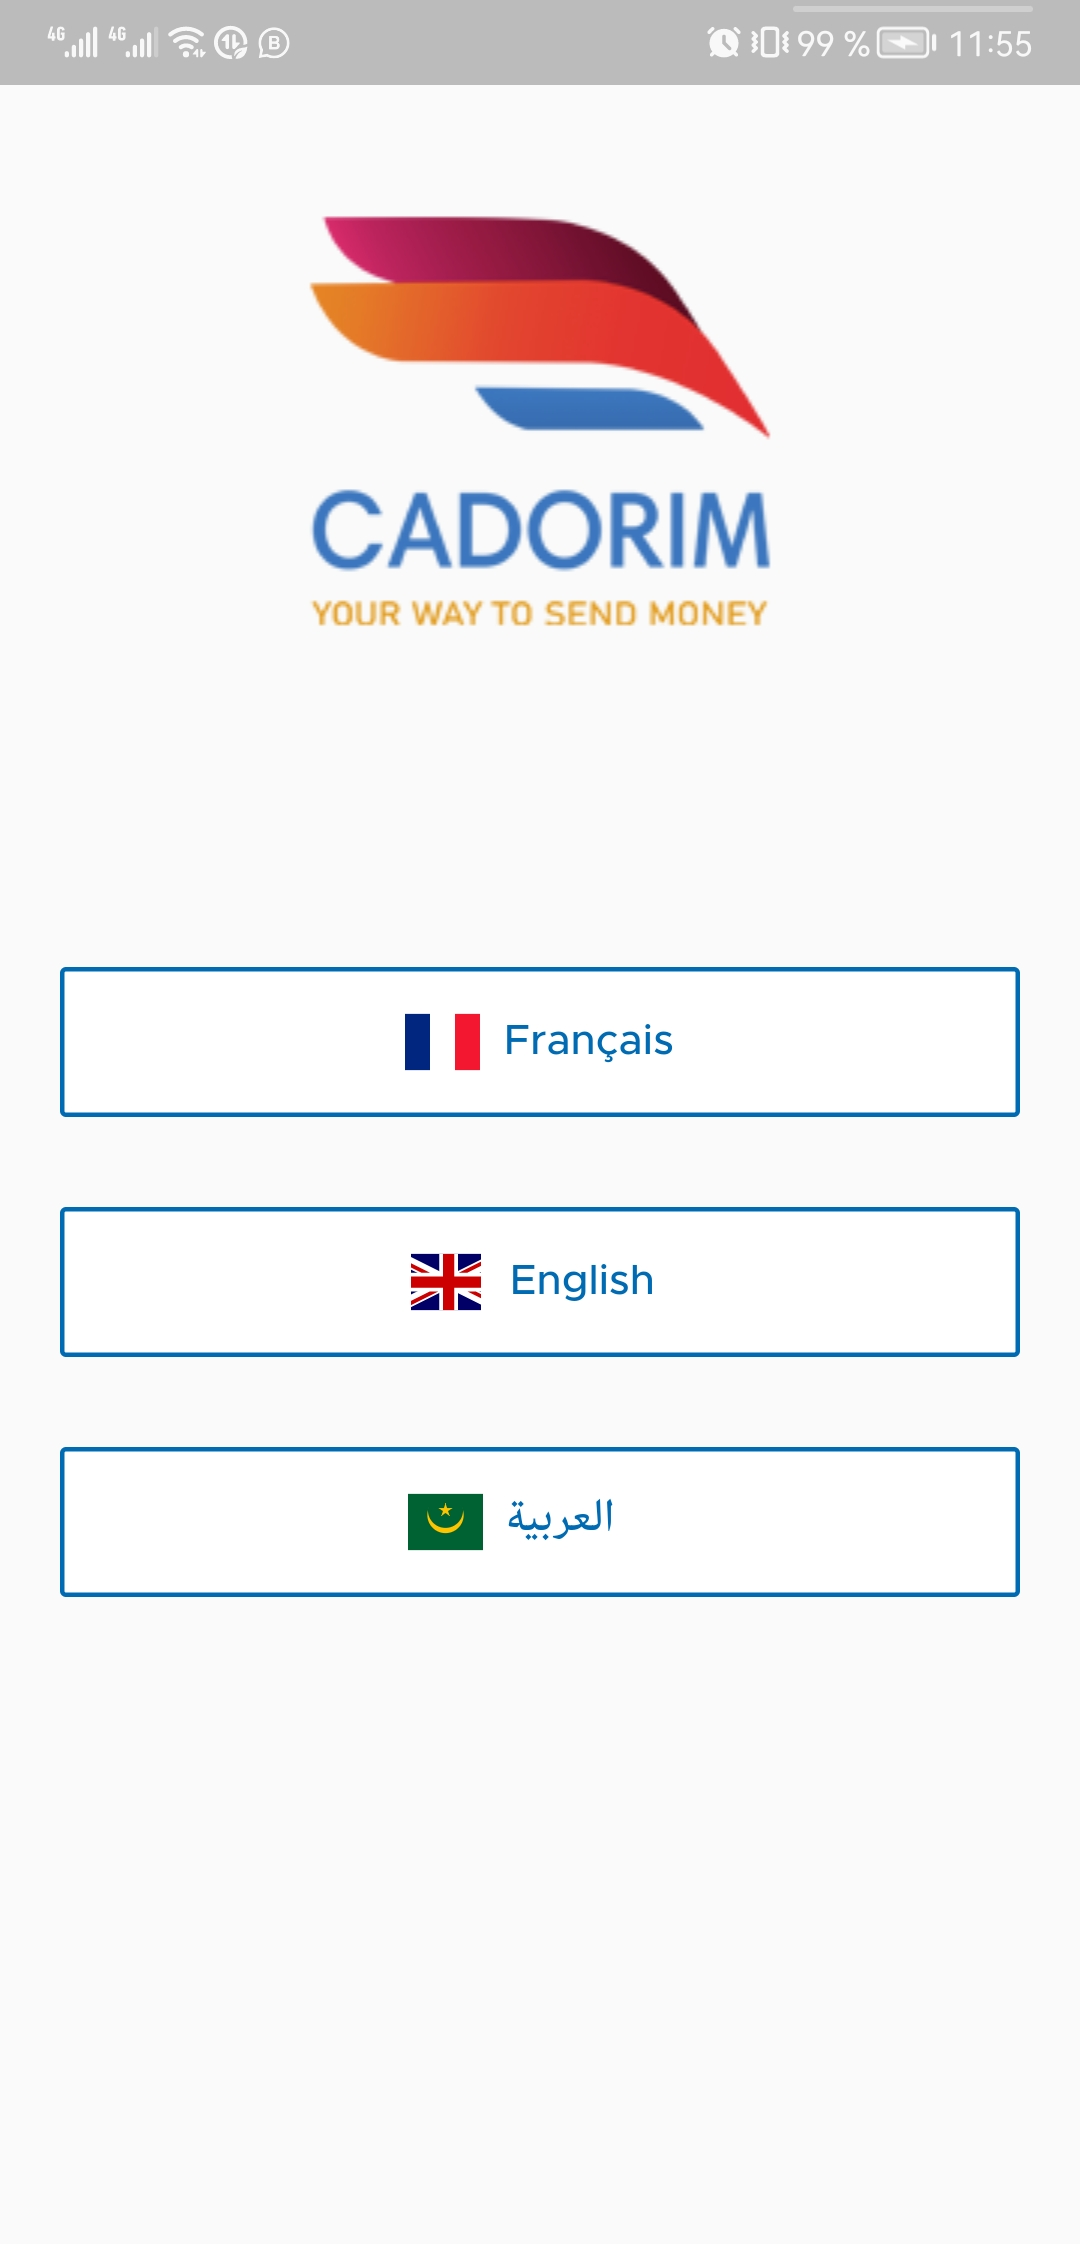
\includegraphics[width=5cm]{./Template LaTeX/Images/1.jpg} }}%
	\qquad	
	\subfloat[\centering  Acceuil]{{
\includegraphics[width=5cm]{./Template LaTeX/Images/2.jpg} }}%
	\caption{Interfaces Accueil}%
	\label{fig:example}%
\end{figure}


	content...

\begin{figure}%
	\centering
	\subfloat[\centering choix de lange ]{{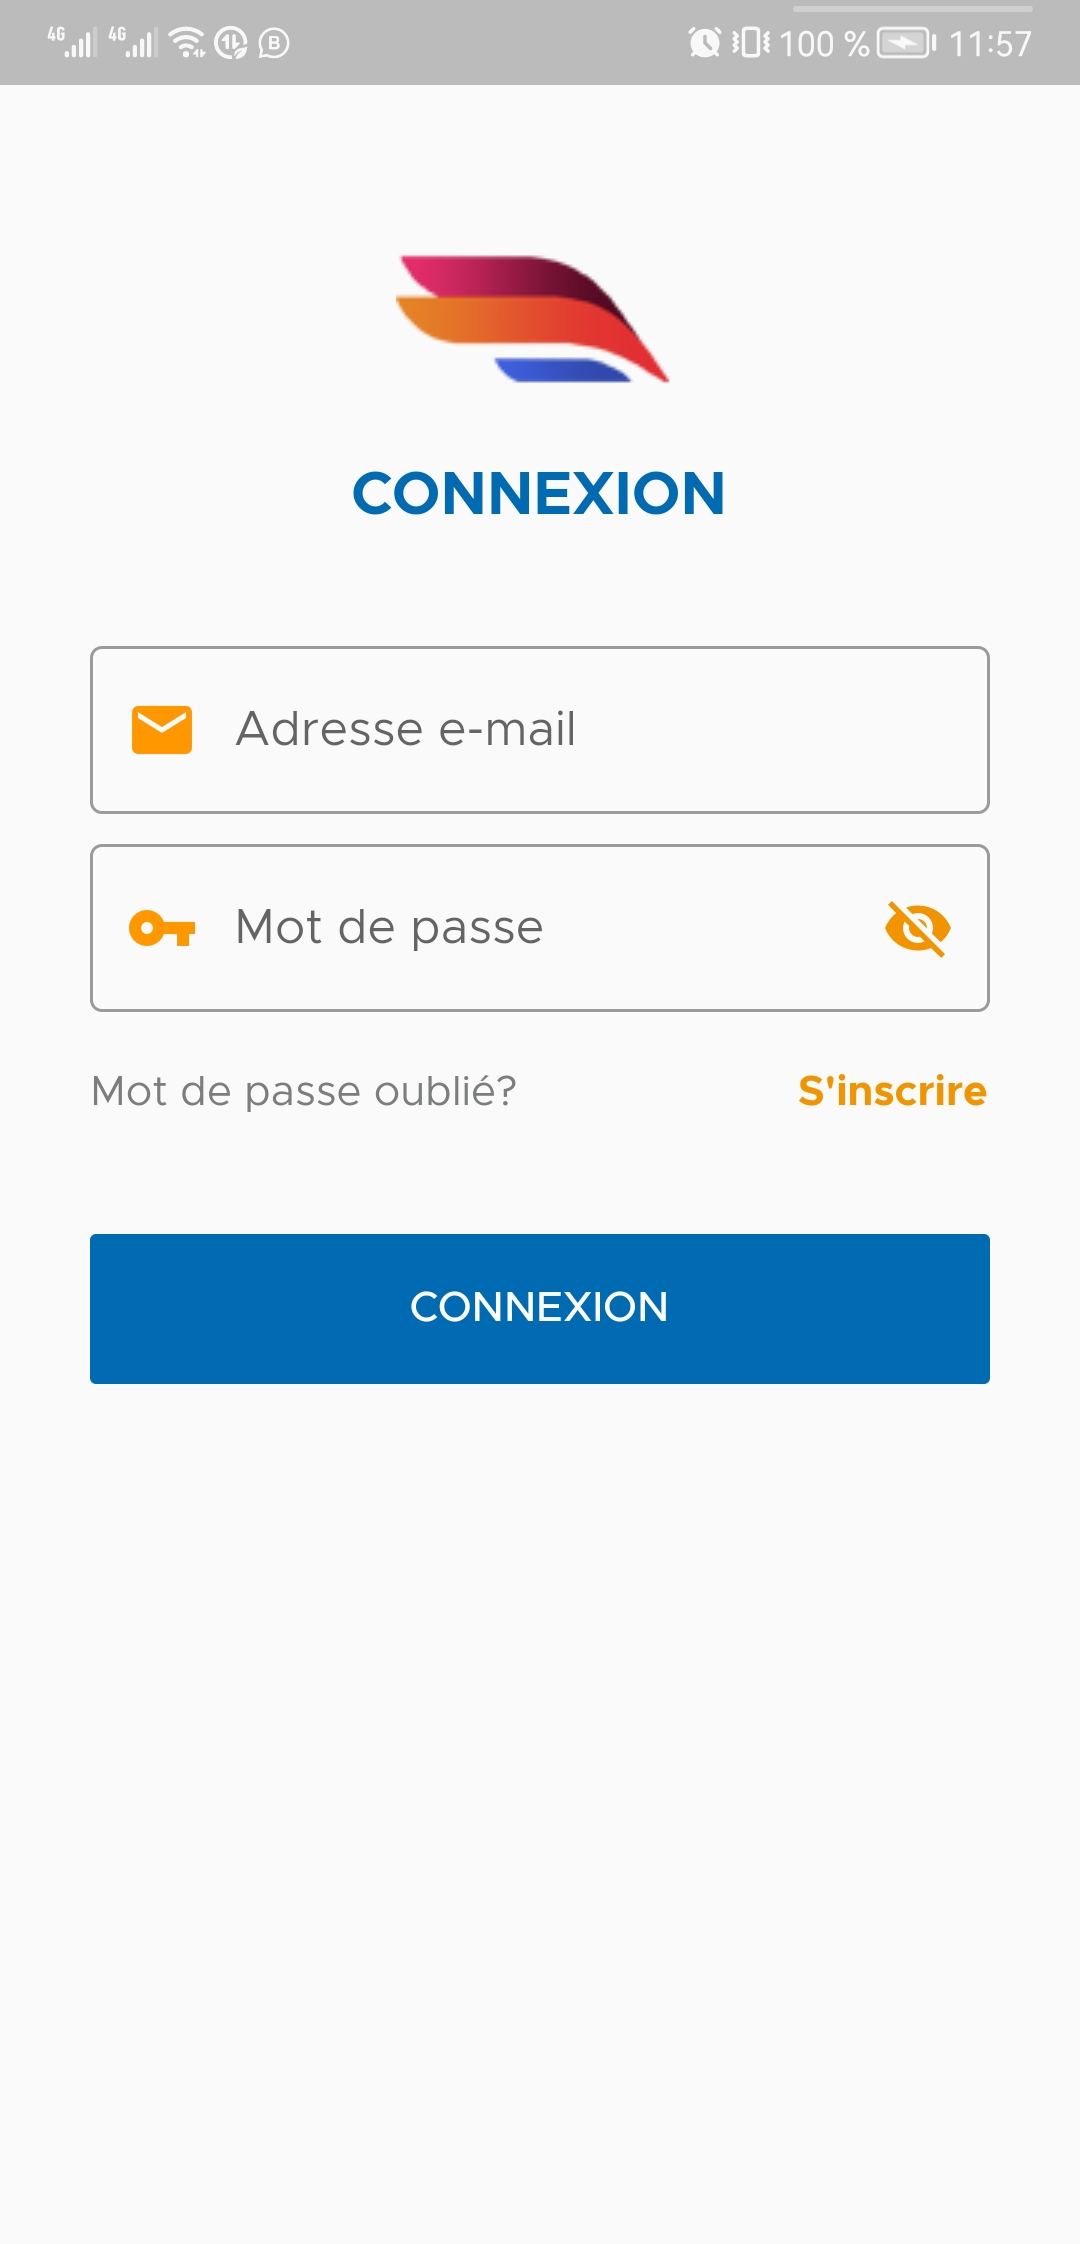
\includegraphics[width=5cm]{./Template LaTeX/Images/3.jpg} }}%
	\qquad
	\subfloat[\centering  Acceuil]{{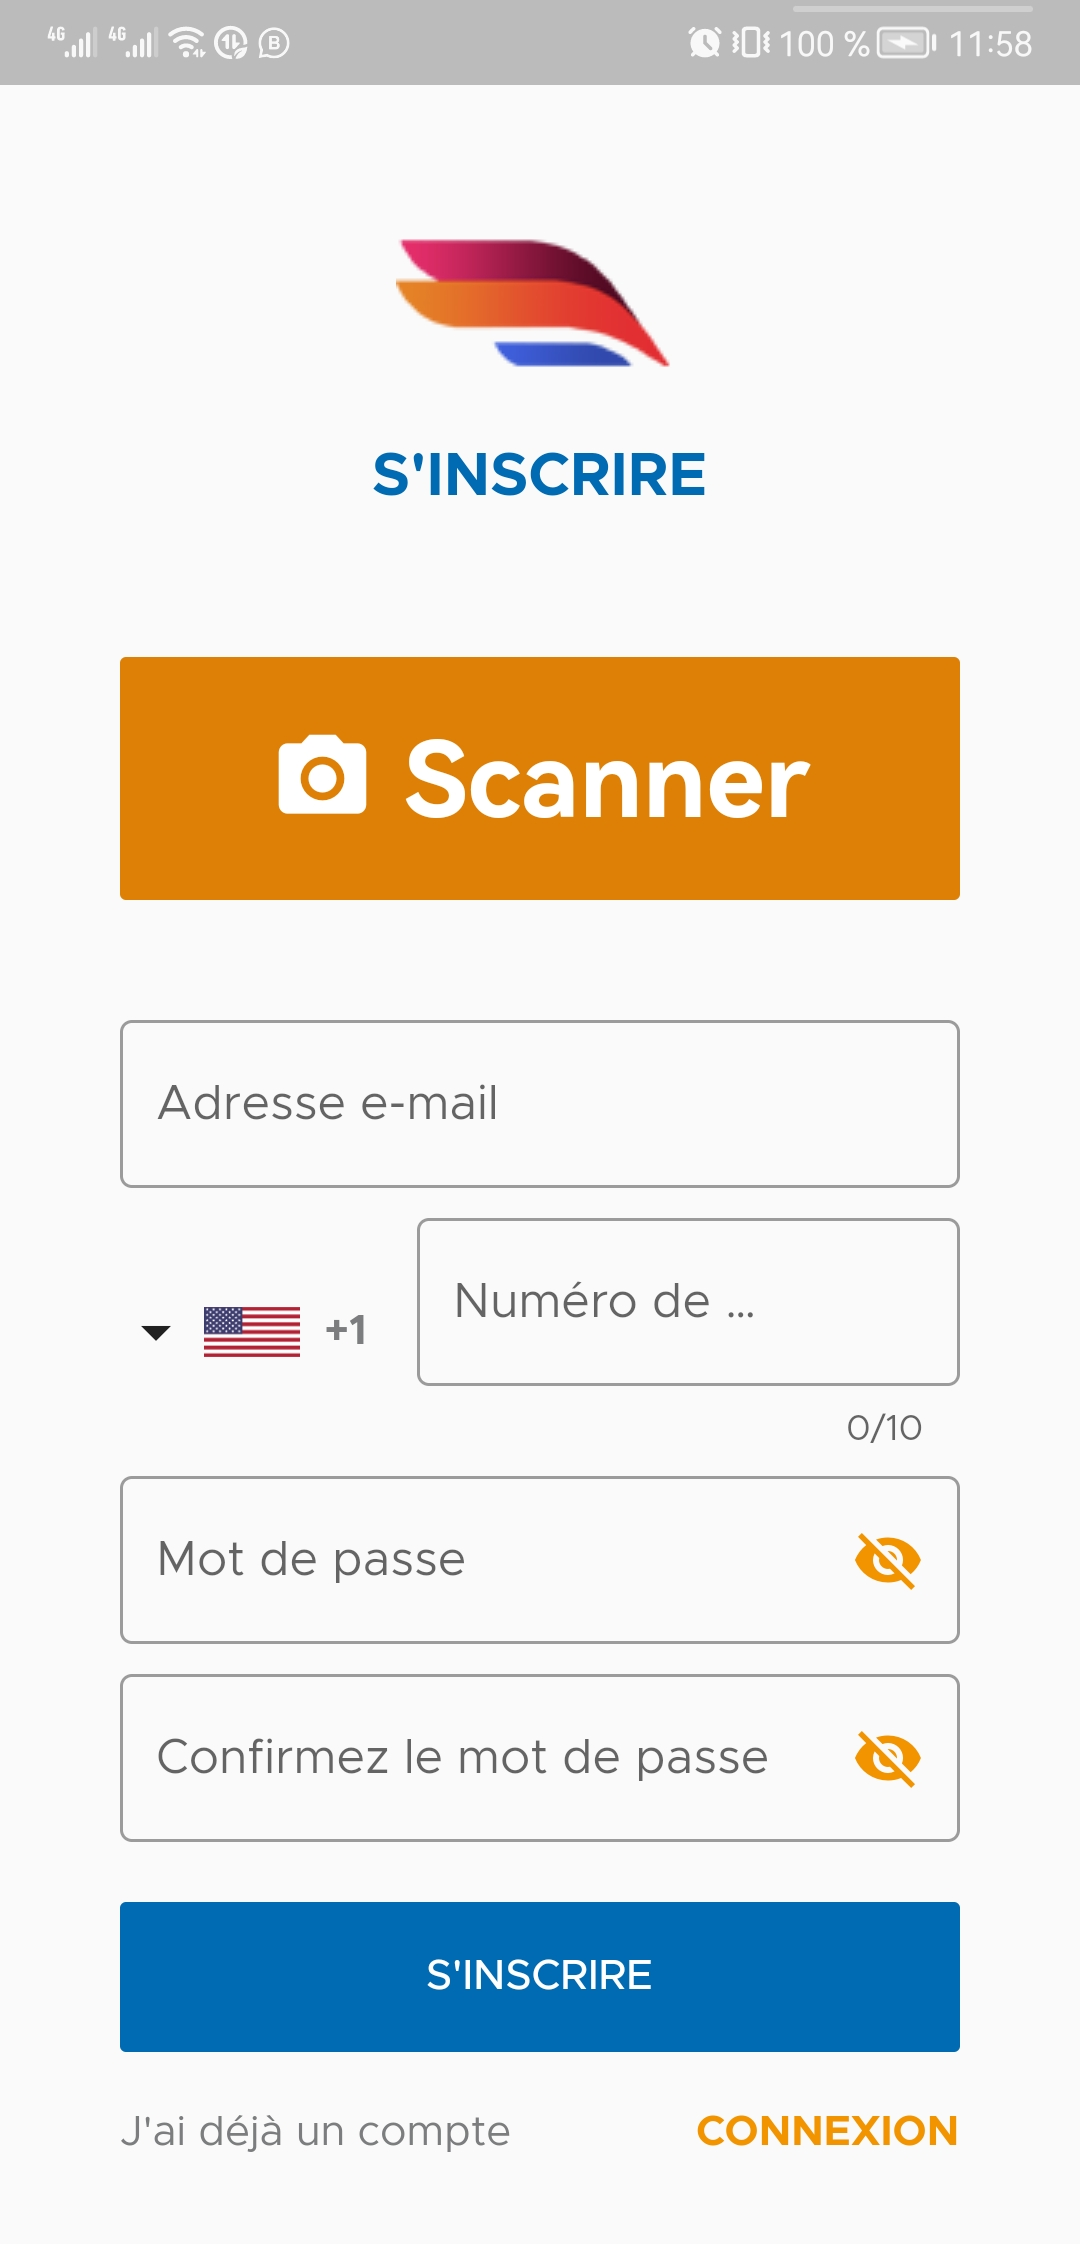
\includegraphics[width=5cm]{./Template LaTeX/Images/4.jpg} }}%
	\caption{Interfaces Accueil}%
	\label{fig:example}%
\end{figure}
\end{comment}
